\documentclass[12pt]{article}
\usepackage[utf8]{inputenc}
\usepackage{geometry}
\geometry{margin=1in}
\usepackage{graphicx}
\usepackage{amsmath}
\usepackage{enumitem}
\usepackage{hyperref}

\title{Chapter 2: Project Goals}
\author{AAI Project Team -- TH Rosenheim}
\date{\today}

\begin{document}

\maketitle

\section{Project Goals}

The goal of this project is to support PSM-Protech in automating the extraction and interpretation of technical data from feasibility reports and scanned documents. The project aims to reduce manual work in data processing and accelerate feasibility analysis by implementing a hybrid pipeline composed of OCR and machine learning components.

This AI-driven solution will consist of:
\begin{itemize}
    \item An \textbf{OCR-based table extraction system} that automatically detects and parses numerical data from scanned documents or image-based PDFs.
    \item An \textbf{image classification module} that supports feasibility validation by recognizing key structural or visual patterns relevant to PSM’s engineering decisions.
\end{itemize}

These capabilities will contribute to the automation of manual review processes in engineering and sales, reduce human error, and improve responsiveness during customer inquiries and project scoping.

\subsection*{Goal Overview}

\begin{table}[ht]
\centering
\begin{tabular}{|p{1cm}|p{8cm}|p{4cm}|}
\hline
\textbf{ID} & \textbf{Goal Description} & \textbf{Success Criteria} \\
\hline
G1 & Automate extraction of tabular numerical data from feasibility reports & Successful OCR extraction on 80\%+ of target fields \\
\hline
G2 & Enable classification of component types from document images & Model achieves 85\%+ classification accuracy on test set \\
\hline
G3 & Integrate OCR and classification into a unified hybrid pipeline & End-to-end pipeline runs with minimal human intervention \\
\hline
G4 & Provide prototype that can be tested by stakeholders at PSM-Protech & Working software demo presented before review deadline \\
\hline
G5 & Document system behavior and architecture & Delivery of readable technical documentation and demo \\
\hline
\end{tabular}
\caption{Project goals and success criteria}
\label{tab:project_goals}
\end{table}

\subsection*{Rich Picture: System in Context}

The following diagram illustrates the high-level interaction between actors (e.g., engineers, sales personnel), systems (e.g., OCR pipeline, document storage), and data flows. It serves to capture the context in which the AI solution will operate.

\begin{figure}[ht]
    \centering
    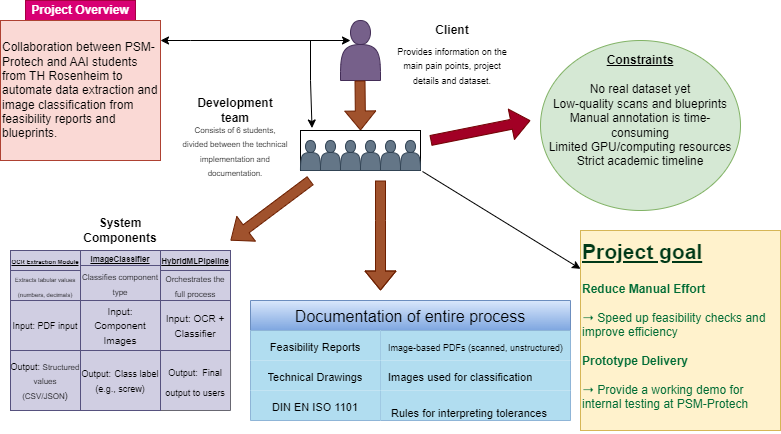
\includegraphics[width=\textwidth]{Rich-Picure.drawio.png}
    \caption{Rich Picture: Overview of system context and stakeholders}
    \label{fig:rich_picture}
\end{figure}

\vspace{1em}
\noindent
In order to ensure that extracted geometric and dimensional values are aligned with industry expectations,
the system should interpret and validate numerical data in accordance with international standards such as
\textit{DIN EN ISO 1101}, which defines rules for geometrical tolerancing of form, orientation, location, and run-out.

\end{document}



